% !TEX encoding = UTF-8 Unicode
\documentclass[BachelorPaper]{subfiles}
\acresetall
%Providecommands für Subfiles
    \providecommand{\citepic}[1]{(#1)}
    \providecommand{\citefig}[2]{(#1, S. #2)}
    \providecommand{\citefigm}[2]{(Modifiziert #1, S. #2)}

\begin{document}
\chapter{Results}
As the results of a software engineering project -- in the most favorable cases -- are functioning software the following paragraphs include display the different project components working together. In the following paragraphs it will be shown how a \ac{MCC} can add a satellite with a single transponder in the administrative interface as well as a \ac{GCC} registering with the \ac{MCC}, and changing his user profile both via the BOINSO MCC Web Client or -- modeling an arbitrary client implementation -- directly via the web \ac{API}. \\

\begin{figure}[!htbp]
\centering
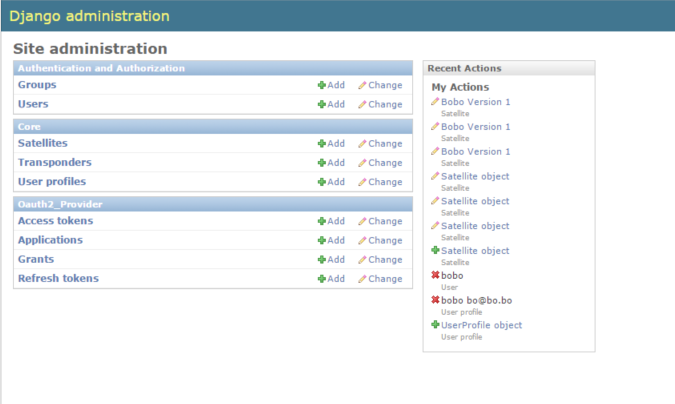
\includegraphics[width=0.96\linewidth]{PICs/BacPics/results/admin_1.png}
\caption{BOINSO Core Web Application main administrative page listing the different modules and tasks}\label{fig:admin_1}
\end{figure}

Figure \ref{fig:admin_1} shows the administrative page of a \ac{MCC} administrator. The different groups separate the installed Django modules. A developer can decide which modules are presented and how they are displayed. The Django administrator pages are extremely extendable and can be configured for the most administrative tasks -- like in this case adding a new satellite.

\begin{figure}[!htbp]
\centering
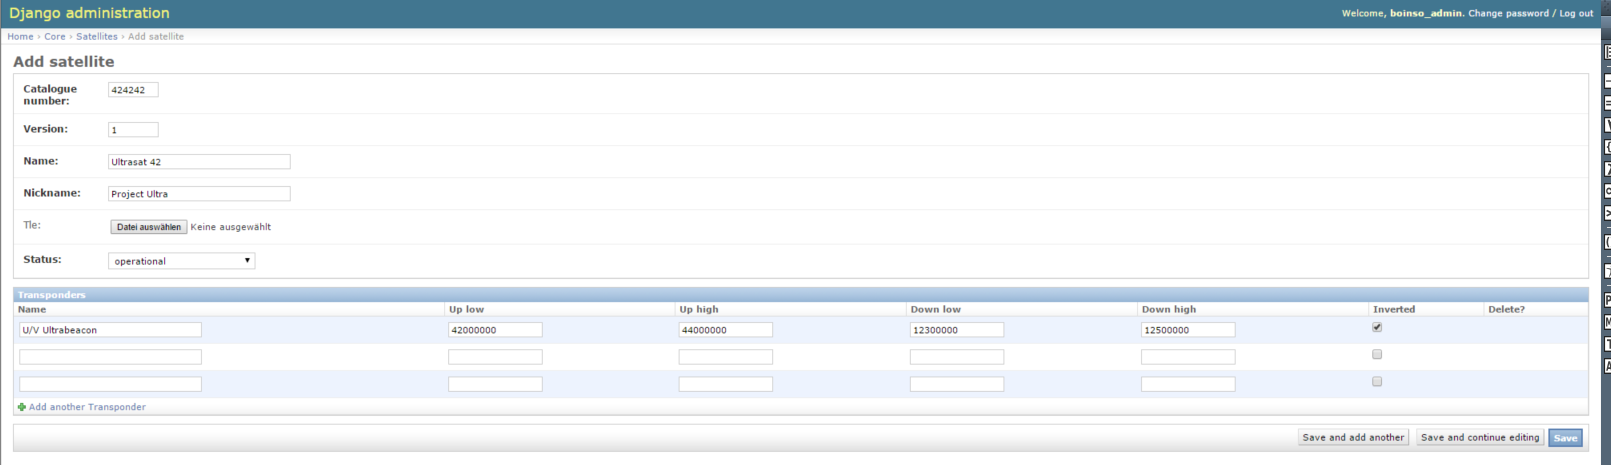
\includegraphics[width=0.96\linewidth]{PICs/BacPics/results/admin_2.png}
\caption{Django admin satellite management form with inline transponder form.}\label{fig:admin_2}
\end{figure}

In figure \ref{fig:admin_2} the form which is used to ad a satellite and its related transponders. The administrative forms are automatically generated by the Django internals after the underlying data model. Inline forms -- like in this case the transponder form -- are not standard Django behavior but an be explicitly set as shown in listing \ref{lst:admin.py} which also shows how other custom modules are registered with the administrative interface. \\

\lstinputlisting[language=Python, caption={Python script explicitly configuring the Django administrative interface}, label=lst:admin.py]{listings/admin.py}

\begin{figure}[!htbp]
\centering
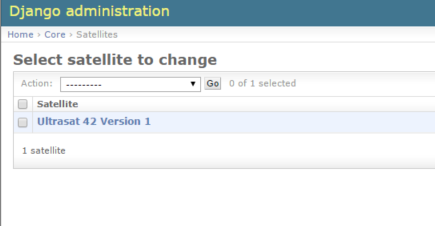
\includegraphics[width=0.96\linewidth]{PICs/BacPics/results/admin_3.png}
\caption{List of existing satellite objects listed by their model representation}\label{fig:admin_3}
\end{figure}

As seen in figure \ref{fig:admin_3} the newly created satellite is listed and can be modified or deleted. Sorting options as well as search fields can also be added to the Django administrative interface. In this case it is not very likely for a \ac{MCC} to have many satellites so the added complexity is not needed. \\

\begin{figure}[!htbp]
\centering
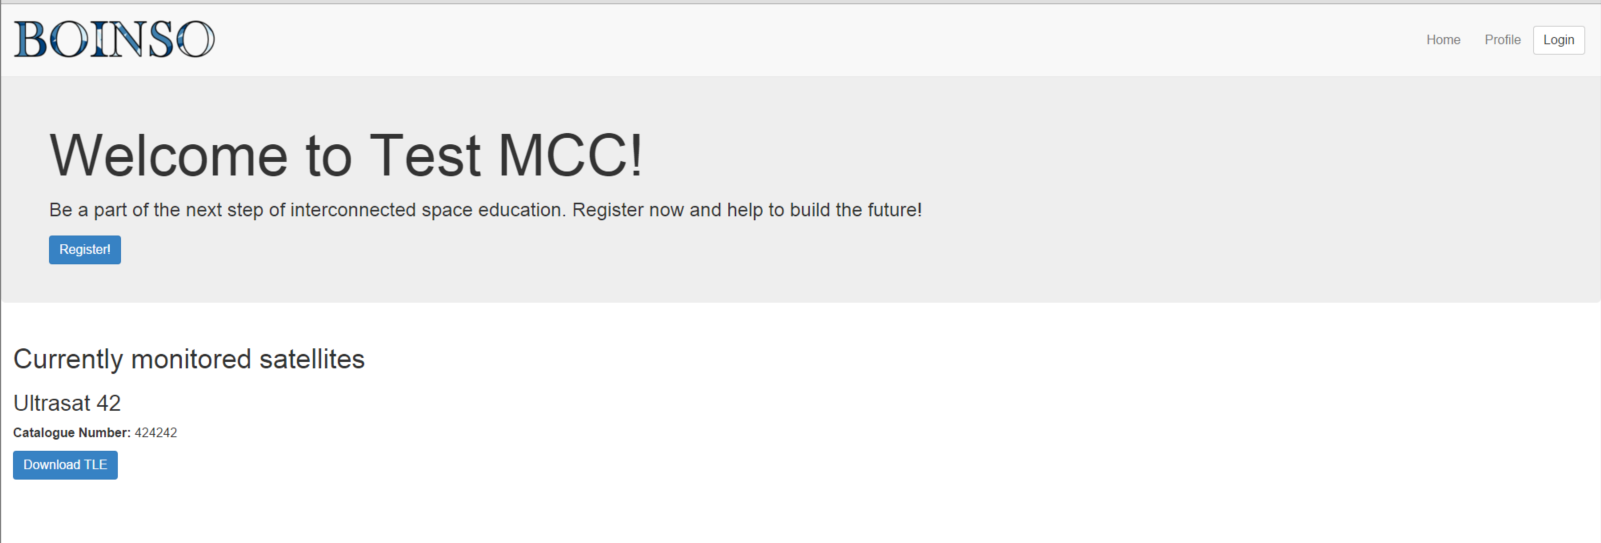
\includegraphics[width=0.96\linewidth]{PICs/BacPics/results/mcc_webapp_1.png}
\caption{BOINSO MCC Web Client homepage}\label{fig:mcc_web_1}
\end{figure}

From a client perspective the main entry point would be the \ac{MCC}'s web page -- in this case modeled by the BOINSO MCC Web Client. Figure \ref{fig:mcc_web_1} shows the homepage where every user is informed about the available satellites as well as motivated to participate. \\

\begin{figure}[!htbp]
\centering
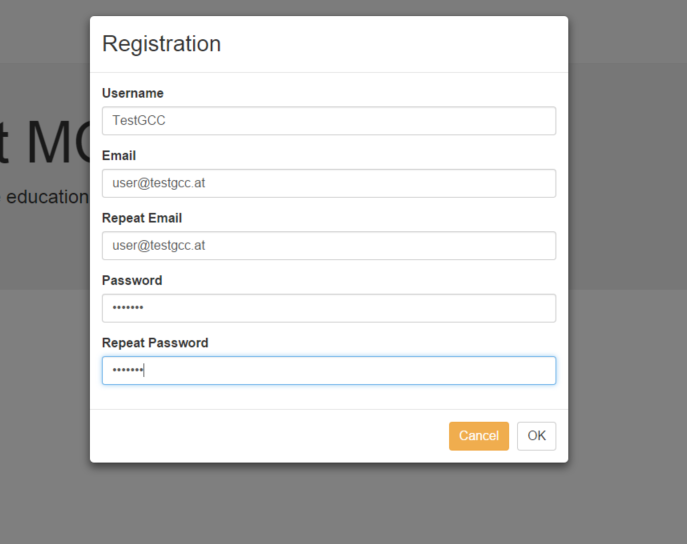
\includegraphics[width=0.96\linewidth]{PICs/BacPics/results/mcc_webapp_2.png}
\caption{BOINSO MCC Web Client registration form}\label{fig:mcc_web_2}
\end{figure}

The registration form as seen in figure \ref{fig:mcc_web_2} collects the most vital information about new users. A successful user creation automatically creates a connected OAuth2 application which provides the client id and the client secret. In the web application those more complex communication steps are hidden from the user. \\

\begin{figure}[!htbp]
\centering
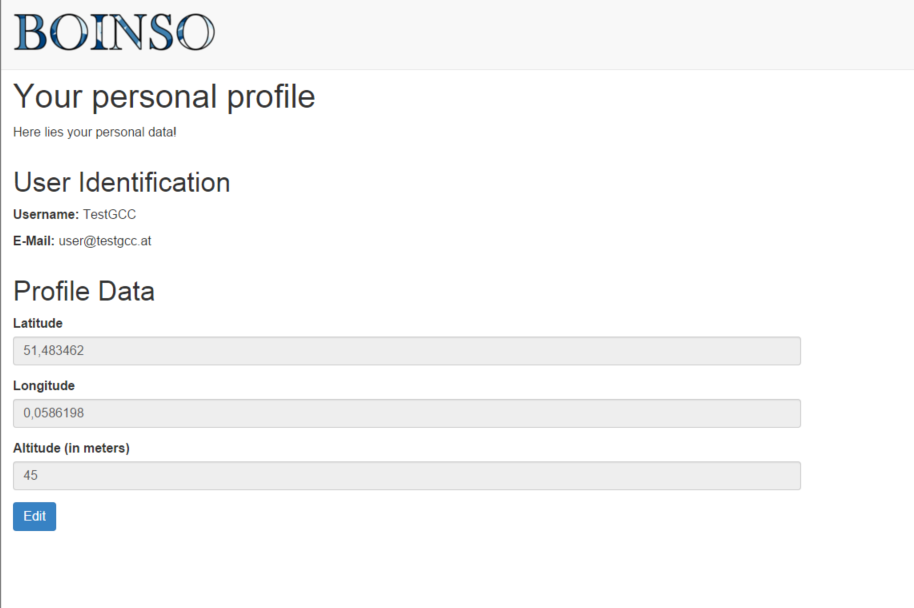
\includegraphics[width=0.96\linewidth]{PICs/BacPics/results/mcc_webapp_3.png}
\caption{BOINSO MCC Web Client profile page}\label{fig:mcc_web_3}
\end{figure}

A logged-in user may access his or her profile page as seen in figure \ref{fig:mcc_web_4}. A user without proper authentication -- this includes registered users with a timed out access token -- are redirected to the home page where the log-in form is opened. \\

\begin{figure}[!htbp]
\centering
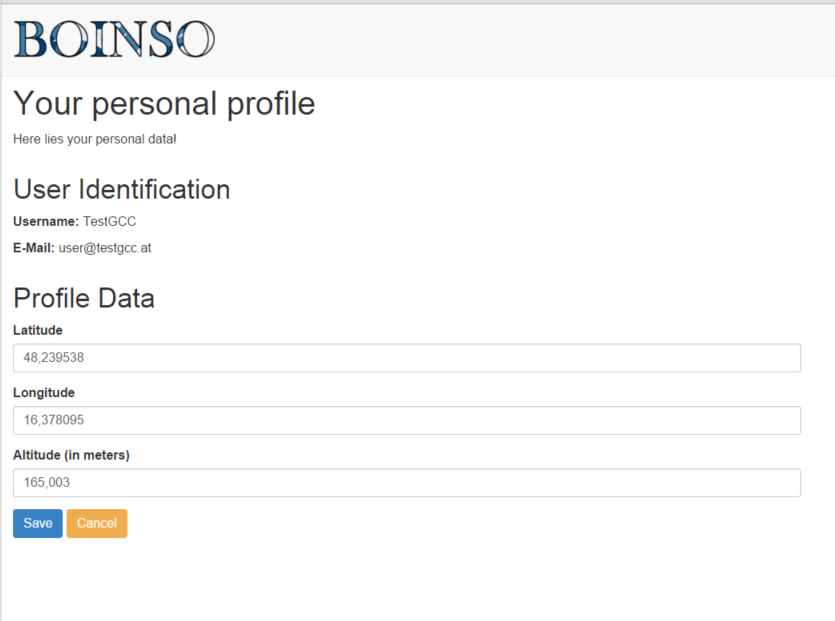
\includegraphics[width=0.96\linewidth]{PICs/BacPics/results/mcc_webapp_4.png}
\caption{BOINSO MCC Web Client profile data management form}\label{fig:mcc_web_4}
\end{figure}

As the initial user profile always includes the geo-location of Greenwich -- just by convention to make the initial registration easier for new users -- users have the possibility to change their profile data as seen in figure \ref{fig:mcc_web_4}. \\

\begin{figure}[!htbp]
\centering
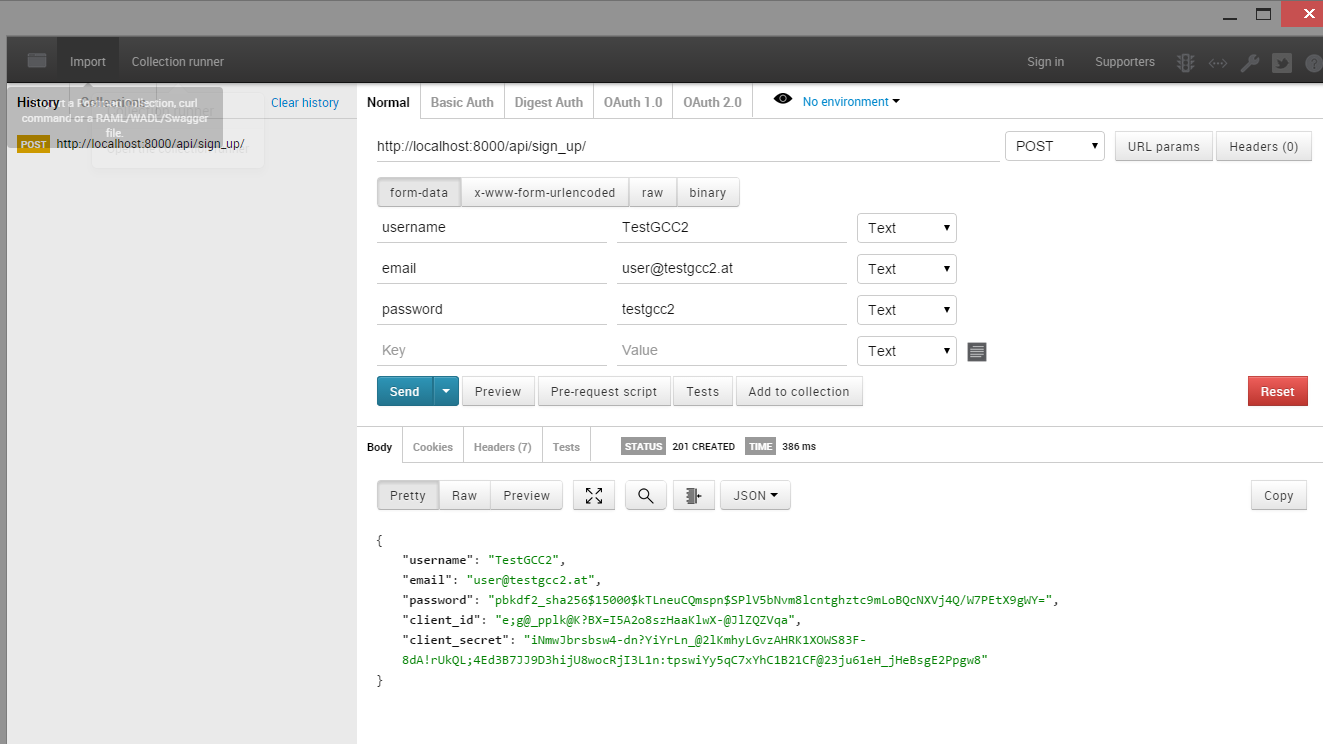
\includegraphics[width=0.96\linewidth]{PICs/BacPics/results/postman_1.png}
\caption{The registration of a new user via Postman}\label{fig:postman_1}
\end{figure}

One of the projects main goals is to give users the possibility to write their own clients -- or fill the gaps between legacy software and the BOINSO network with middleware as we did with the BOINSO GPredict Bridge. To simulate an arbitrary client the \ac{REST} \ac{API} testing tool Postman was used. The registration process is a straight forward POST call to the related \ac{API} endpoint as seen in figure \ref{fig:postman_1}. \\

\begin{figure}[!htbp]
\centering
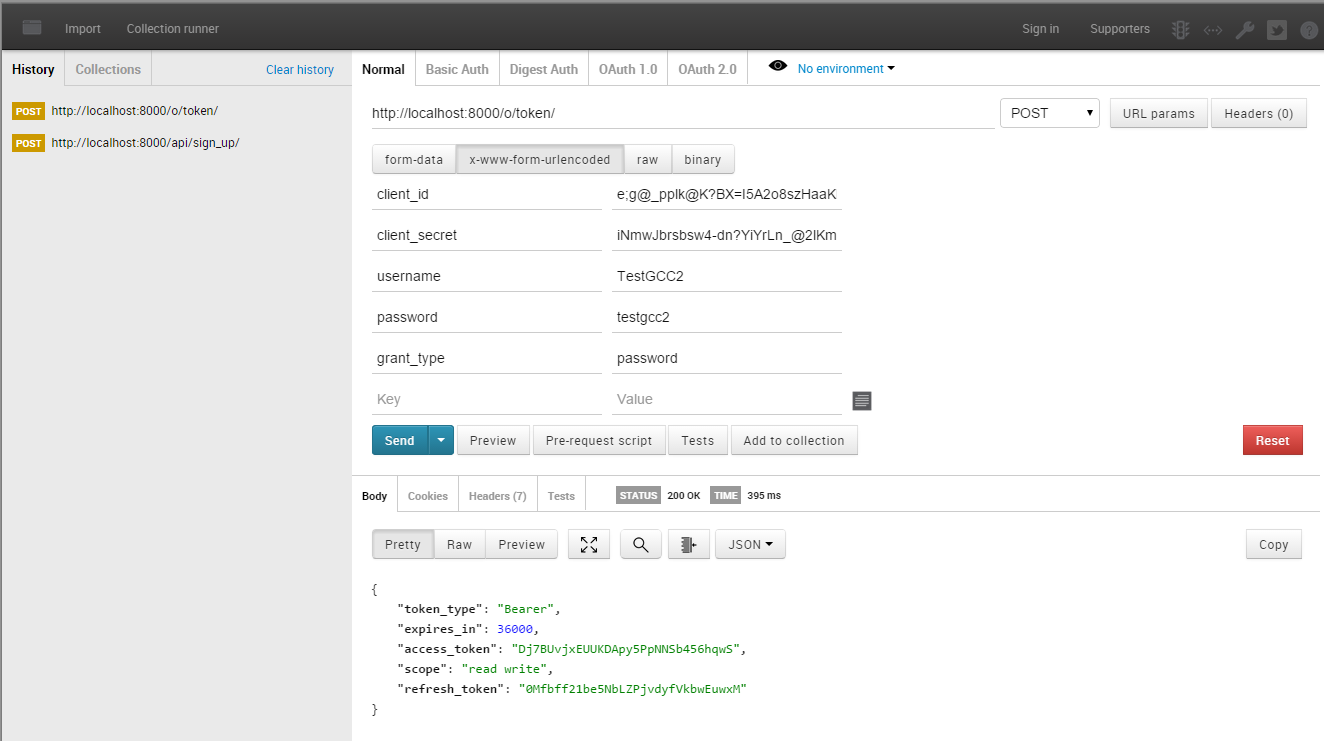
\includegraphics[width=0.96\linewidth]{PICs/BacPics/results/postman_2.png}
\caption{Retrieval of the user OAuth2 access token via Postman}\label{fig:postman_2}
\end{figure}

As seen in figure \ref{fig:postman_1} the response to the registration includes both the client id as well as the client secret. In combination with the user name and user password a call to the \ac{URL} of the OAuth2 provider endpoint -- implemented by the Django OAuth Toolkit -- results in the retrieval of a distinct authentication token (with a limited lifetime) as seen in figure \ref{fig:postman_2}. \\

\begin{figure}[!htbp]
\centering
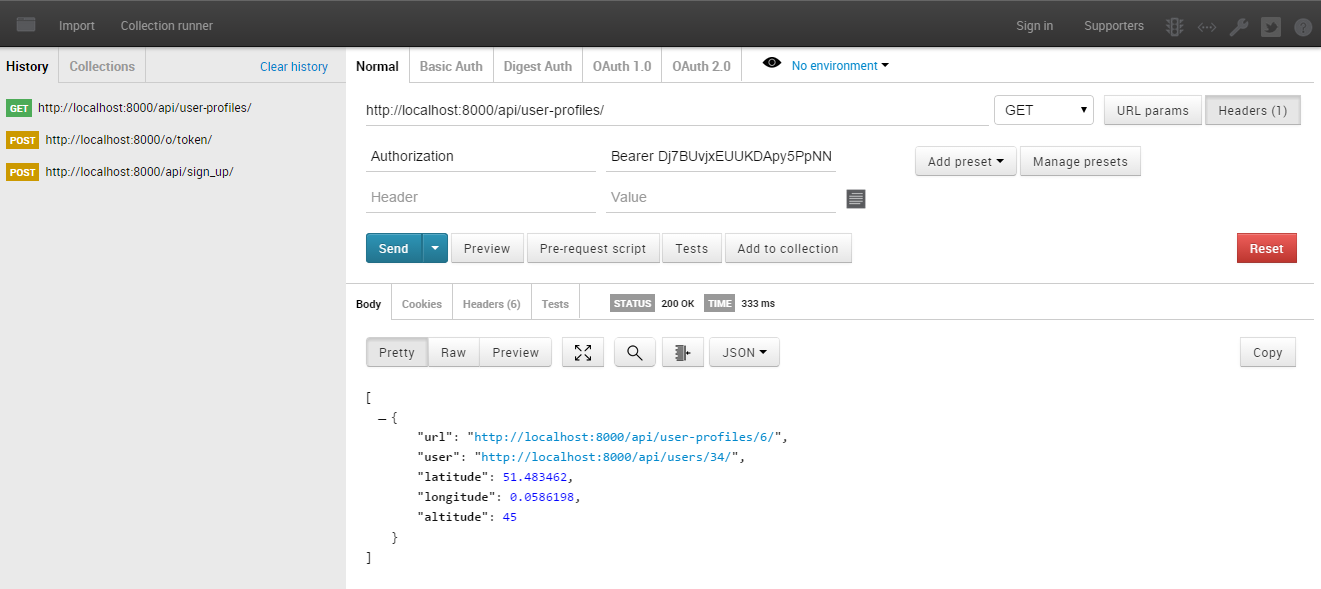
\includegraphics[width=0.96\linewidth]{PICs/BacPics/results/postman_3.png}
\caption{Retrieval of the user profile belonging to the OAuth2 authentication token}\label{fig:postman_3}
\end{figure}

As user credentials tend not to change often client designers are not encouraged to safe them after accessing a user token as a lost token can be rather retrieved rather easily whereas lost credentials impose a major security threat. Figure \ref{fig:postman_3} proves that the OAuth2 token -- assumed it is neither timed out nor lacking bearer rights -- is enough to retrieve a user's profile. \\

\begin{figure}[!htbp]
\centering
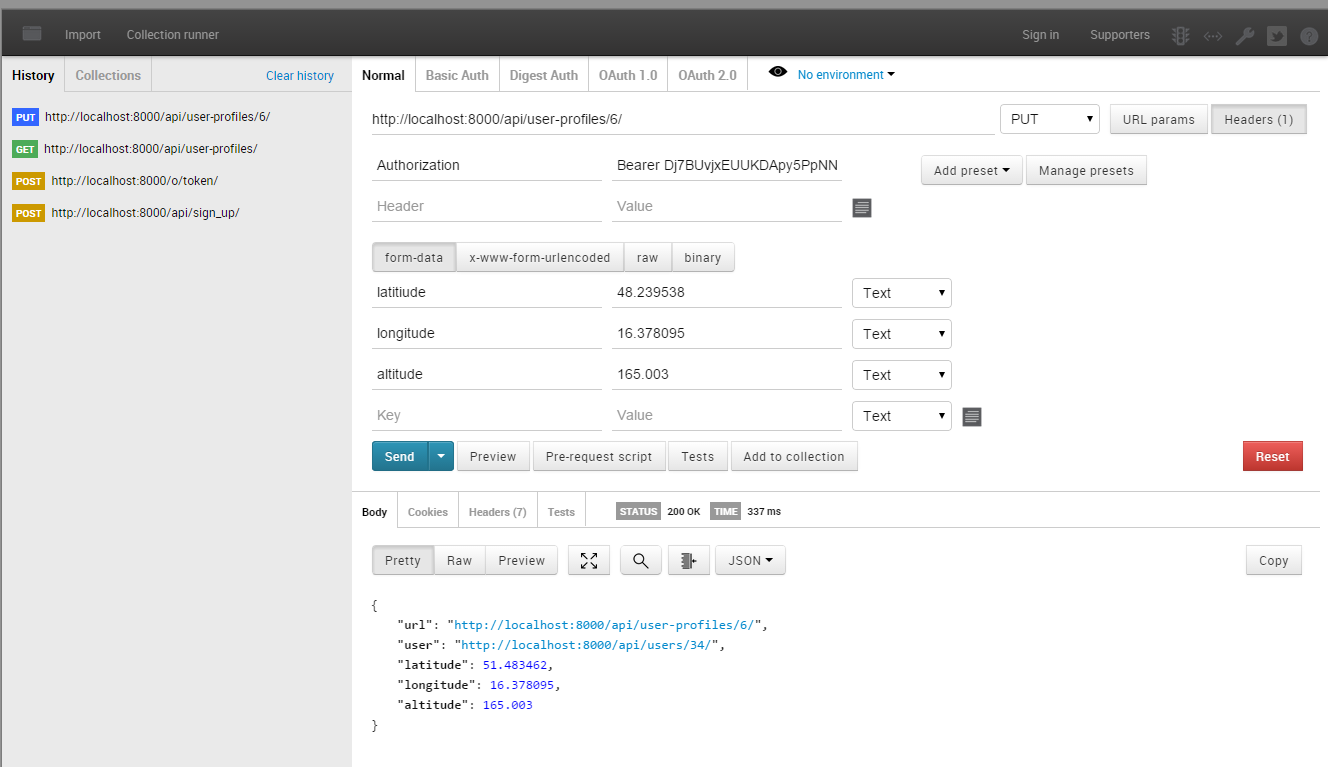
\includegraphics[width=0.96\linewidth]{PICs/BacPics/results/postman_4.png}
\caption{Update of a distinct user profile via Postman}\label{fig:postman_4}
\end{figure}

Finally the information about the retrieved user profile -- the user profile url field -- can be used as the next endpoint, proving the conceptual benefits of \ac{HATEOAS} in action. Using the \ac{HTTP} verb PUT new information -- as long as they are in a valid format -- can be directed at the user profile endpoint resulting in updated user profile values as seen in figure \ref{fig:postman_4}.

\end{document}